%!TEX root = ../template.tex
%%%%%%%%%%%%%%%%%%%%%%%%%%%%%%%%%%%%%%%%%%%%%%%%%%%%%%%%%%%%%%%%%%%%
%% chapter3.tex
%% NOVA thesis document file
%%
%% Chapter with a short latex tutorial and examples
%%%%%%%%%%%%%%%%%%%%%%%%%%%%%%%%%%%%%%%%%%%%%%%%%%%%%%%%%%%%%%%%%%%%

\typeout{NT FILE chapter3.tex}%


\chapter{Related Work}
\label{cha:related_work}

This chapter presents research works that were considered related to this thesis theme.
These studies were selected based on their relevance to the concepts described in Chapter \ref{cha:fundamental_concepts}, including Geographic Information System (\gls{GIS}) integration, \gls{3D} modelling, spatial databases, and virtual tours.

\section{The Turin 1911 Project}
\label{sec:turin_project} 

\subsection*{General Overview}

The "Turin 1911: The World's Fair in Italy" is a research project~\cite{article} conducted by the \textit{University of California San Diego} and  \textit{Politecnico di Torino} where a multidisciplinary team cooperates to document and investigate the 1911 World’s Fair held in Turin.
It integrates archival research, \gls{3D} reconstruction, and web\gls{GIS} technology to study and preserve the architectural and Cultural Heritage (\gls{CH}) of the Fair\footnote{\url{https://arcg.is/1HfSqG}}.

\subsection*{Process Description}

The web\gls{GIS} and \gls{GIS}-\gls{BIM}\footnote{\url{https://www.autodesk.com/solutions/aec/bim}} web apps are interactive tools to digitally navigate and query the environment. 
Three types of elements were used to create a \gls{3D} web\gls{GIS}: polygonal feature class, multi-patch feature class, or \gls{3D} object.

The historical map of the \textit{Valentino Park Fairground} was georeferenced and digitized, and a \gls{2D}/\gls{3D} map interface was developed using ArcGIS Online\footnote{\url{https://www.arcgis.com/index.html}}, allowing users to switch between views seamlessly. 
To develop the \gls{3D} models in the \gls{BIM}-\gls{GIS} Web App, not only, photographs of each object, but also, plans, elevations, and sections of some Built Environment Objects, were collected. Using technical drawings, \gls{3D} models were generated and compared with historical photographs.
The final web\gls{GIS} application, for both dimensions, was created using ArcGIS Experience Builder\footnote{\url{https://www.esri.com/en-us/arcgis/products/arcgis-experience-builder/}} configurable widgets (Figure \ref{fig:turin_study}).

\subsection*{Interactive Features}

Several tools were developed in the web\gls{GIS}, including a search bar, an option for switching between a \gls{2D} map and a \gls{3D} scene, a layer list, a legend, navigation controls, filters, and pop-ups, allowing users to explore built environment objects. 
\gls{BIM} was used for detailed \gls{3D} reconstruction of selected Fair pavilions (e.g., Pavilion of Siam), and to create an interactive \gls{3D} scene with those layers. 
The actual shape of \textit{Valentino Park} was created from an aerial photogrammetric survey and processed in Agisoft Metashape\footnote{\url{https://www.agisoft.com/}}. Applications like Experience Builder
enhanced interactivity, offering features like navigation and measurement tools, bookmarks, layer toggles, and camera orientation. The current geolocation feature enables users in the park locate themselves on the web\gls{GIS} and web app. 
The digitized archival materials are catalogued and linked to the geometries in a dedicated Geospatial Database. 
 

\begin{figure}[h!]
  \centering
  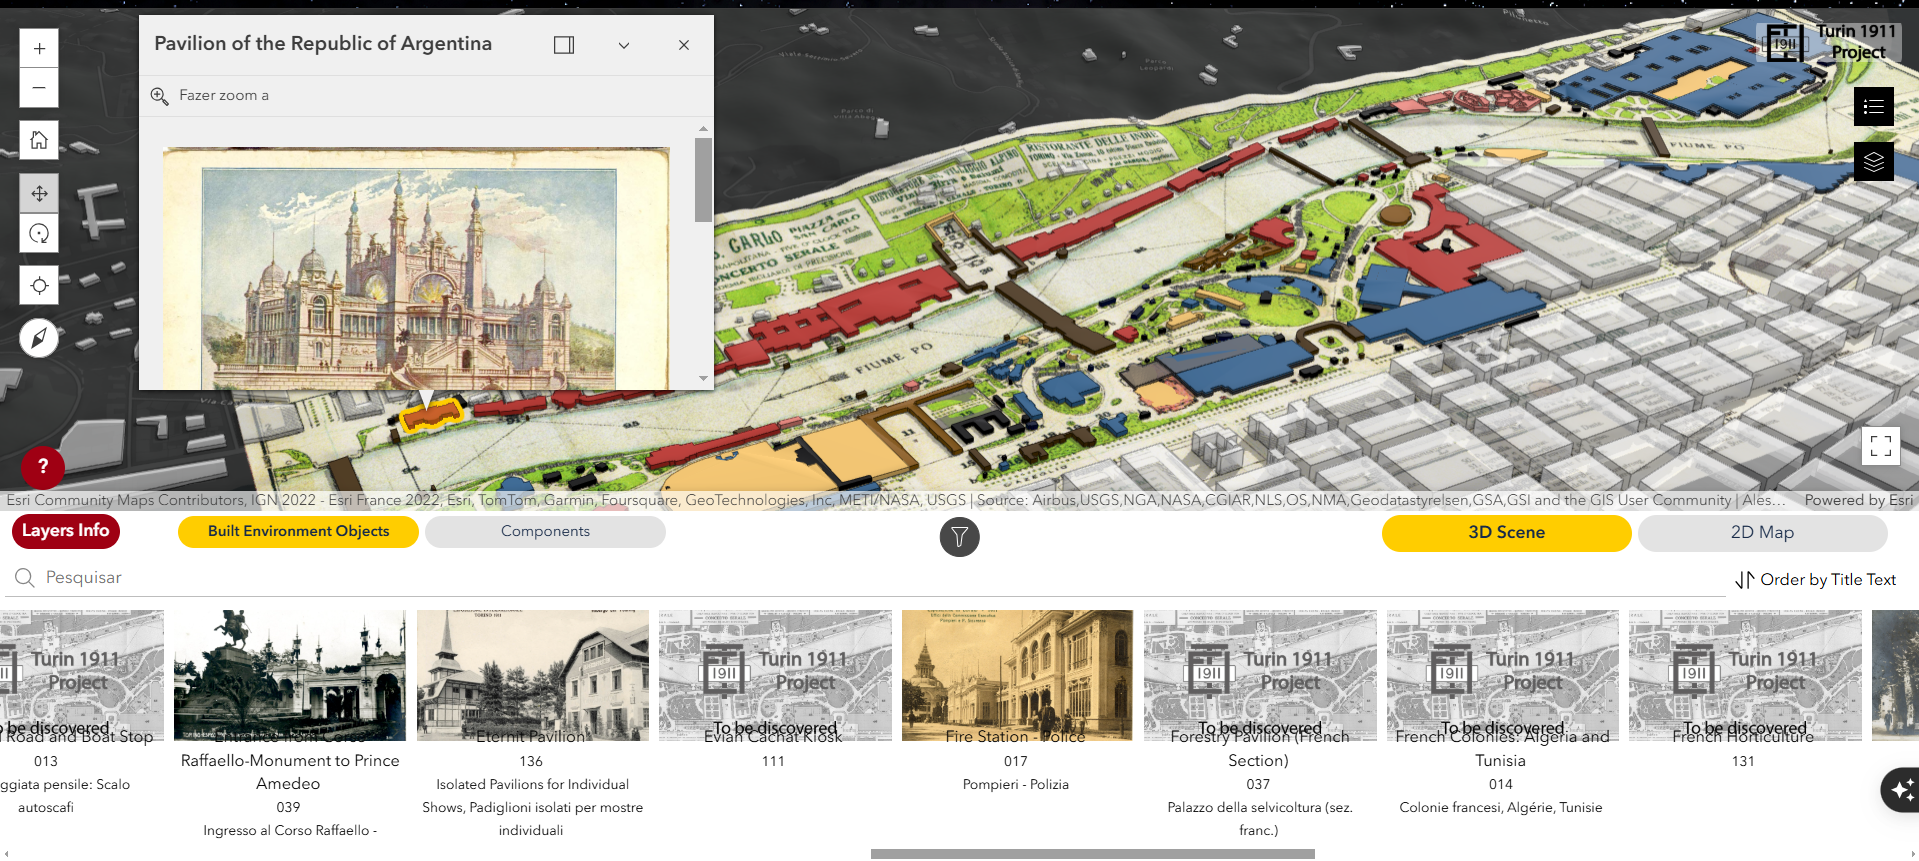
\includegraphics[width=0.8\linewidth]{turin_study}
  \caption{The web\gls{GIS} application. \small{Displayed functionalities:} \footnotesize{bottom left – search bar and objects list; top left – navigation controls and a pop-up; bottom right – 3D scene/2D map buttons; top right – map legend and layer control buttons.}}
  \label{fig:turin_study}
\end{figure}
\vspace{-10pt}
\section{Web-Based \gls{GIS} for \gls{CH} of Safranbolu, Turkey} 
\label{sec:gis_safranbolu}

\subsection*{General Overview}

This study~\cite{arca2018development} focuses on the documentation and preservation of the \gls{CH} of Safranbolu, Turkey, a UNESCO World Heritage site\footnote{\url{https://whc.unesco.org/en/list/614/}}. 
The goal of this project is to establish an internet-based information system and the modelling for GIS of all historical constructions of Safranbolu historical city.
This will be accomplished by compiling documentation and preservation of \gls{CH}, using \gls{GIS}, \gls{3D} models and digital photogrammetry.

\subsection*{Process Description}

The development of this work started with digital photogrammetry, where the objects coordinate system was defined, and control points marked on the ancient artefacts, and photographs of the antiquities taken.

Pictures then were transferred to computer and evaluated with photogrammetric software (\textit{Photomodeler}\footnote{\url{https://www.photomodeler.com/}}). Following this, the \gls{3D} modelling of the historical buildings was executed.
\gls{3D} of the building were obtained using photos from photogrammetry taken from different views, and the object models were covered with different surface and image textures.
\gls{GIS} was used to analyse spatial objects, such as buildings constructed within parcels and roads. Land parcels were represented as polygons, while roads with polylines.
The city map of Safranbolu was obtained in \gls{CAD}\footnote{\url{https://www.autodesk.com/pt/solutions/cad-software}} format, and then transferred to ArcGIS. This data was then evaluated in \gls{GIS} by building a topological infrastructure.
In the next phase of the project, all collected data—such as photos, videos, architectural drawings, and \gls{3D} and \gls{VRML}~\cite{713310} models—related to the selected historical buildings was prepared. 

\begin{figure}[h!]
  \centering
  \begin{subfigure}[b]{0.45\textwidth}
      \centering
      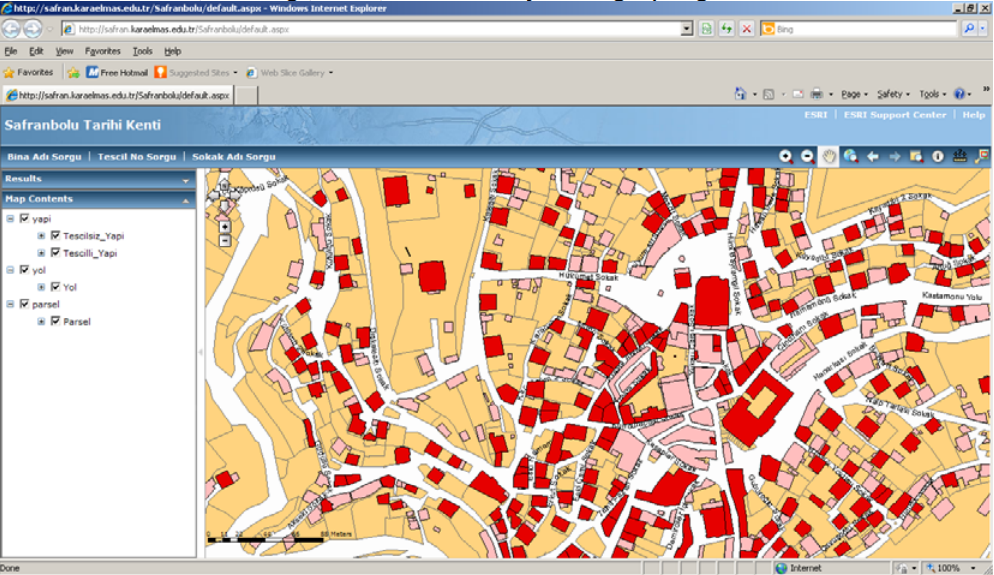
\includegraphics[width=1.0\textwidth, height=4cm]{turkey_thesis}
      \caption{Registered and non-registered buildings in the old Safranbolu area.}
      \label{fig:x}
  \end{subfigure}
  \hfill
  \begin{subfigure}[b]{0.45\textwidth}
      \centering
      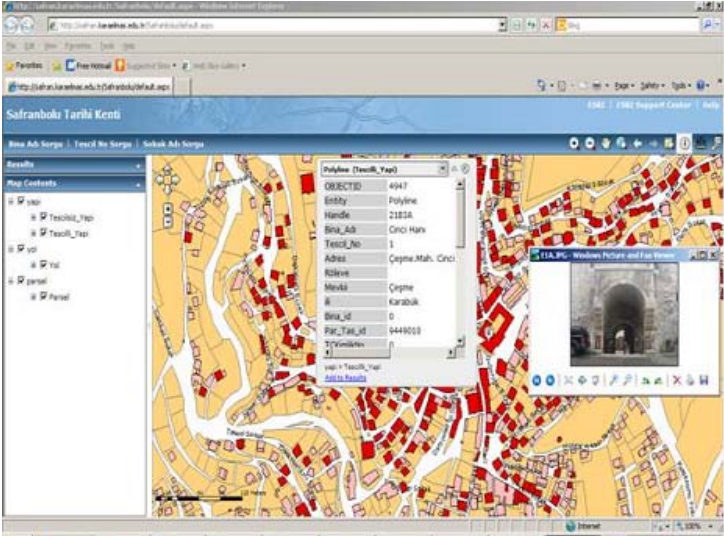
\includegraphics[width=1.0\textwidth, height=4cm]{test}
      \caption{Designed Web-based \gls{GIS} \textit{Cinci Caravanserai}.}
      \label{fig:y}
  \end{subfigure}
     \caption{Illustrative views of the Web-\gls{GIS} application.}
     \label{fig:z}
\end{figure}
\FloatBarrier

This project integrates spatial data (e.g., building locations and \gls{3D} images) with non-spatial data (e.g., textual descriptions and historical information about the buildings) to document the historic town of Safranbolu. 
Through the interface (Figure \ref{fig:z}), users can visualize various types of data, including land parcels, registered and non-registered buildings, roads, ownership details, addresses, and other relevant details about cultural monuments in the old Safranbolu area.

\section{\gls{VR} Scenario with Funerary Artifacts from Ancient Egypt} 
\label{sec:3d_vr_devices}

\subsection*{General Overview}

This research~\cite{gonizzi20153d} leverages \gls{VR} to enhance the accessibility and understanding of Egyptian funerary artefacts in the Sforza Castle, Milan. 
Aimed at exhibition renewal, the project creates an immersive \gls{VR} experience to engage visitors of the “Archaeological Museum” in Milan, with the ancient Egyptian "Path of the Dead" ritual, integrating interactive \gls{3D} models and hieroglyphic translation tools. 
Four key funerary artefacts were selected for their historical and archaeological significance: the Ushabty statuettes (representing a pharaoh or minister), the Heart Scarab amulet, and the Wooden Sarcophagus.

\subsection*{Process Description}

Firstly, the photogrammetry survey was built by moving the camera all around these objects to capture all angles. Subsequently, the software \textit{Agisoft Metashape} was used for texture blending. Then, the output file was imported into \textit{Adobe Photoshop}\footnote{\url{https://www.adobe.com/pt/products/photoshop.html}} for word delineation, outlining and identification. 
Finally, \textit{Polyworks}\footnote{\url{https://www.innovmetric.com/products/products-overview}} was used to simplify the model, and in resolution/texture optimization.
The \gls{VR} device Oculus Rift DK2 provided stereoscopic visualization, while Leap Motion\footnote{\url{https://www.ultraleap.com/}} tracked hand movements for object interaction (grabbing, rotating, and highlighting).

Responsive Points of Interest (\gls{POI}) created in the context of the project, were exported in \textit{fbx}\footnote{\url{https://www.autodesk.com/products/fbx}} format, and the cut parts of the artefacts were then imported to Unity\footnote{\url{https://unity.com/}}, for integration as \gls{3D} models.
These \gls{POI} highlight cultural symbols and texts on artefacts (e.g., religious inscriptions). When selected, they provide detailed descriptions and explanations.
The computer graphics program \textit{\gls{3D} Studio Max}\footnote{\url{https://www.autodesk.com/pt/products/3ds-max}} was used to enhance specific elements of the models, to improve hieroglyphs readability.
Touch-Triggered Transliteration and Translation allows users to interact with hieroglyphic symbols(Egyptian writing). 


\begin{figure}[h!]
  \centering
  \begin{subfigure}[b]{0.45\textwidth}
      \centering
      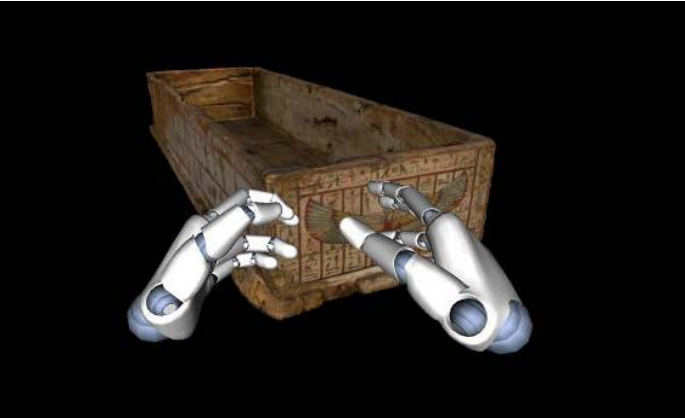
\includegraphics[width=1.0\textwidth, height=4cm]{vrGis_thesis1}
      \caption{Grabbing and rotating the object.}
      \label{fig:vrGis_thesis1}
  \end{subfigure}
  \hfill
  \begin{subfigure}[b]{0.45\textwidth}
      \centering
      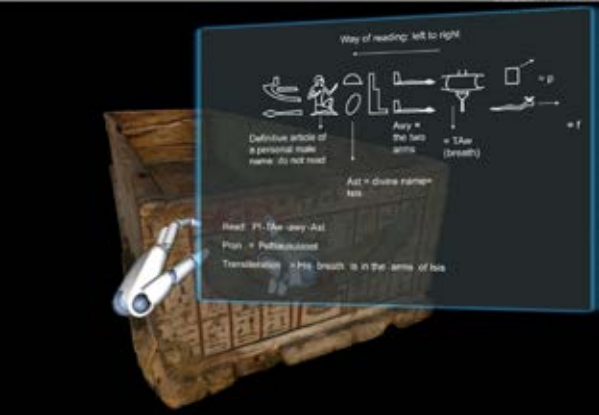
\includegraphics[width=1.0\textwidth, height=4cm]{vrGis_thesis2}
      \caption{Highlighting and translation the text.}
      \label{fig:vrGis_thesis2}
  \end{subfigure}
     \caption{Visual representations of the implemented \gls{VR} scenario}
     \label{fig:vrGis_thesis}
\end{figure}

If the user wants to know more about these words, they can touch them, and the word is automatically enhanced and the transliteration and the following translation appear as illustrated in Figure \ref{fig:vrGis_thesis2}. The data involved is the name of the deceased, and descriptions explaining images or drawings on the objects.
Users can rotate and grab the \gls{3D} models using hand gestures, as shown in Figure \ref{fig:vrGis_thesis1}.
\FloatBarrier

\section{Related Work developed at NOVA LINCS}
\label{sec:thesis_nova}

At NOVA, recent research work has been consistently focused on developing digital tools for museums and cultural institutions, aiming to offer immersive experiences through \gls{VR} technology or \gls{3D} media visualizations 
of \gls{CH} objects, often incorporating interactive maps, an approach to be implemented in this dissertation. Over the past year, two Master of Science theses~\cite{tese_tourCoimbra2024,tese_tourFaria2024}  have explored how to 
present a virtual tour of museums. Vilar's thesis~\cite{tese_jogosVilar2022} explored interactive games and \gls{3D} models, with an emphasis on cultural artefacts from the Portuguese Évora site. 
The final thesis~\cite{campanha2024heritage} focuses on \gls{3D} object manipulation, which may be integrated into this dissertation.


\subsection{System for Creating and Exploring Interactive Narratives and Games}
\label{sec:thesis1_nova}

Vilar developed his research thesis work~\cite{tese_jogosVilar2022} as part of the PASEV\footnote{\url{https://pasev.hcommons.org/}} Project \gls{PASEV}. 
The main objective of the project was to analyse new perspectives regarding the cultural manifestations in UNESCO patrimonial city, Évora,
which has a significant historical context~\cite{vilar2024extended}. The project started by Rosário~\cite{rosario2021responsive} and was extended by Ferreira~\cite{Ferreira2021} which were mainly dedicated to the development of a historical soundscape's web platform\footnote{\url{https://pasev.uevora.pt/}}. 
This work focused on the study of sound events that occurred from 1540 to 1910 with the aim of preserving the city's auditory heritage~\cite{rodrigues2021using}. The user can
visualize and display audio and media(including, in some cases, 360º photos and videos) in the web platform.

Vilar expanded the existing \gls{PASEV} platform by introducing JoNI, an infrastructure designed to support the creation of interactive games, involving motivational techniques, such as interactive narratives, gamification structures and the use of \gls{AR}. In the end of this project, a mobile 
application was developed incorporating games with a narrative and characters, including \gls{2D}/\gls{3D} models and auditory data, and object recognition via photos. Two 
functional prototypes supported by the platform were developed. The first, an interactive card game that teaches children about historical music instruments available at the Evora Museum\footnote{\url{https://www.visitevora.net/en/evora-museum/}} using audio and visual elements. The second, a gamified app to promote the discovery 
of diverse locals with their itineraries. Along the route, textual content, videos, audios and a ranking progress are reproduced to generate an interactive and learnable experience. 
For each game, two main tabs were implemented for managing the map and \gls{AR} features of the game. 

This implementation includes \gls{AR} and geolocation technologies to immerse users in Évora's \gls{CH}.
The solution was built on top of an existing base map. Afterward, the \gls{POI} of Évora were identified and represented with \gls{AR} markers. Additionally, GPS tracking was
integrated to allow users to monitor their location.
The solution integrates a native Android environment and Unity game engine for seamless communication. The main goal of this dissertation is the dissemination of the \gls{CH} 
and soundscape of Évora, with the solution integrated into Museu Nacional Frei Manuel do Cenáculo (MNFMC)\footnote{\url{https://www.cm-evora.pt/locais/museu-nacional-frei-manuel-do-cenaculo/}}. 
The database was extended using PostgreSQL and PostGIS technologies.

\subsection{Designing and implementing a museum Virtual Tour, Museu dos Coches}
\label{sec:thesis2_nova}

Coimbra~\cite{tese_tourCoimbra2024} developed a \gls{VE} that simulates a museum visit, providing an immersive and interactive user experience. The project integrates a \gls{3D} environment 
with \gls{3D} scanned objects, complemented by an intuitive and user-friendly interface. 
This virtual tour was based on the National Coach Museum\footnote{\url{http://museudoscoches.gov.pt/pt/}} and performs as a model for \gls{VR} museum environments. This approach can revolutionize 
museum tours, suggesting an alternative, immersive, and innovative platform for cultural enrichment. 
The technologies used include Unity to create and deploy the \gls{VE}, and the virtual visit requires a \gls{VR} headset equipped with hand-tracking capabilities. For this purpose, 
the Meta Quest 3 Headset \footnote{\url{https://www.meta.com/quest/quest-3/}} was used to improve the processing power over earlier models. Therefore, this software ensures an optimized \gls{VR} experience. 
Coimbra's thesis was developed in 2024 and has some points in common with this one. Both use digital tools for an interactive user experience with \gls{CH} elements.


\subsection{Web integration of virtual museums tours and \gls{3D} media visualization, Academia das Ciências}
\label{sec:thesis3_nova}

Last year, Faria~\cite{tese_tourFaria2024} developed his dissertation work in collaboration with \textit{Academia das Ciências de Lisboa}\footnote{\url{https://www.acad-ciencias.pt/}}, one of the oldest scientific institutions in Portugal, active since 1779.
The academy is dedicated to promoting and preserving \gls{CH}, with both physical and digital collections accessible to the public~\cite{academiaCiencias2024}.
The project focuses on integrating \gls{CH} objects in \glspl{VE}. As part of this work, a website was created to provide a virtual tour of the academy, presenting its spaces and \gls{CH} objects in an engaging and informative manner.
This website is available at the following\footnote{\url{https://visita3d.acad-ciencias.pt/}}.
Designed with a user-friendly interface, the website offers an intuitive navigation experience, including an audio guide with simulated narration, background music, a \gls{3D} viewer, enabling the user to explore the components and history behind each artefact.
The project also incorporates an interactive itinerary map, displaying all the available rooms and buttons for instinctive control of the tour. This feature allows users to explore the academy's diverse spaces quickly and effectively.
Matterport\footnote{\url{https://matterport.com/}} technology was employed to create the visualization and interaction environments, providing \gls{3D} spatial mapping of the academy's rooms. Complementing this, \gls{3D} object models were created and displayed in a Sketchfab\footnote{\url{https://sketchfab.com/}} viewer. 
To support these features, several technologies were used, including Matterport Pro3 Camera\footnote{\url{https://matterport.com/pro3}} for the \gls{3D} scanning and 360º immersive views, along with frontend and backend frameworks, including Vue.js\footnote{\url{https://vuejs.org/}} and Tailwind CSS\footnote{\url{https://tailwindcss.com/}} for the interface, 
while the backend relied on Node.js\footnote{\url{https://nodejs.org/}}. In addition, a database to store and manage the media content was implemented.

\subsection{Developing support for digital representations of Heritage artefacts in cultural exhibitions}
\label{sec:marcia_thesis}

Campanha's thesis~\cite{campanha2024heritage} aimed to extend the work of Nunes~\cite{nunes_thesis}, by enhancing user interaction with 
artefacts in \gls{VE}. The functionalities implemented in this work focus on object interaction, such as the ability to apply different textures, the possibility to manipulate specific parts of a \gls{3D} object independently, and access detailed information regarding these parts.
Users can manipulate objects through the three axes (X,Y,Z) by rotating, scaling, or translating them within the virtual space.
To obtain detailed information of the antiquities, the user simply selects the desired component.
Additionally, users can upload the digital \gls{3D} representation of the object to the virtual exhibition and view a gallery menu displaying multiple perspectives of the \gls{3D} models associated with the same artefact.
The system allows users to apply different textures to individual object components and select specific parts, which are outlined with their associated descriptions.
The full interface, including these interactive features, can be observed below in Figure \ref{fig:marcia_image}.

\begin{figure}[h!]
  \centering
  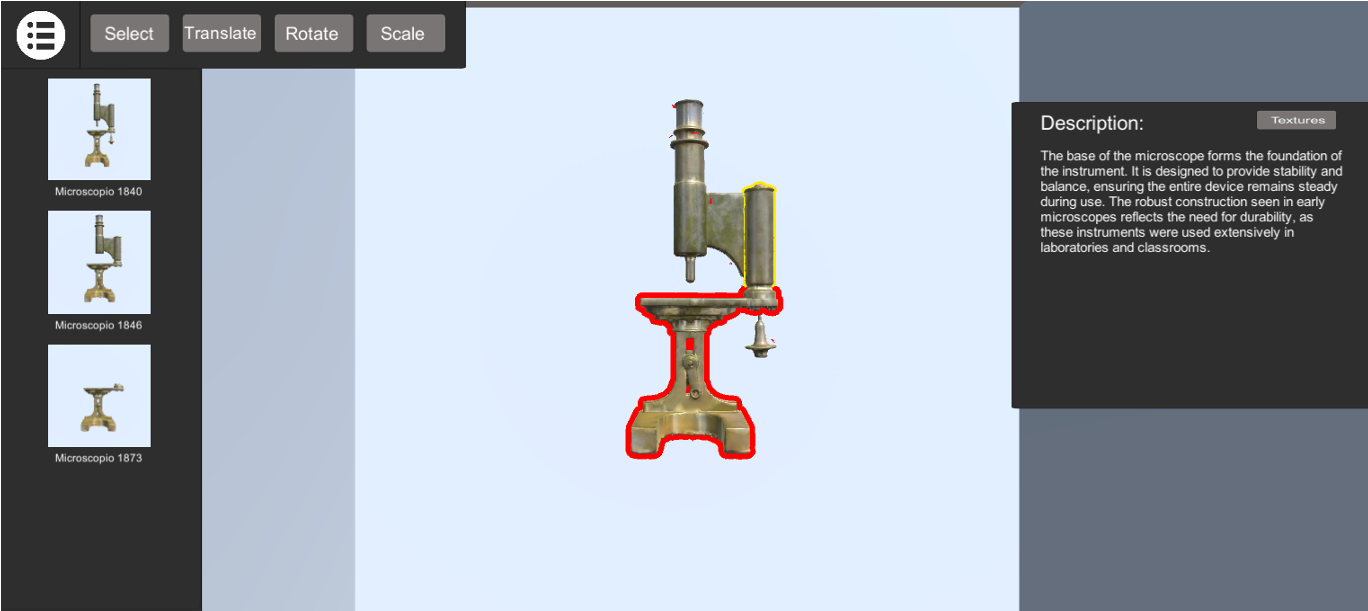
\includegraphics[width=0.8\linewidth]{marcia_thesis}
  \caption{Interface for interacting with heritage artefacts.}
  \label{fig:marcia_image}
\end{figure}
\FloatBarrier

\section{Discussion}
\label{sec:discussion}

This section compares various recent research works and their relevance to this dissertation by analysing their components and contributions. Table \ref{tab:comparison2} provides an illustration of these comparisons.

The "Turin 1911 Project" integrates an interactive map with multiple functionalities, while incorporating \gls{3D} models and a spatial database. Similarly, the Safranbolu \gls{GIS} project focused on the preservation of an archaeological site, using \gls{3D} modeling to map historical buildings and integrating \gls{CH} monuments as metadata relevant to the site. Both projects illustrate the use of \gls{3D} models and digital tools for documentation and preservation. 
However, while these studies remain primarily centered on mapping and geospatial analysis, other research has expanded the focus towards immersive \gls{VR} visualization, as the following \gls{VR} scenario study.
The described project, integrated \gls{VR} to provide an immersive environment, enabling users to interact with valuable artefacts from ancient Egypt. Features such as zooming, scaling, Egyptian writing translation, highlighting, and object manipulation were implemented to enhance the user experience.

To include contemporary Portuguese projects relevant to this research, Section \ref{sec:thesis_nova} was added, exploring digital representations of cultural artefacts, and the dissemination of archeological sites and institutions.
The following three projects integrate a virtual tour. Primarily, \gls{PASEV} project extends an existing historical soundscape web platform by integrating \gls{AR}. This work also incorporates 3D interactive models, a digital map, and was selected due to its completeness and the use of technologies, such as PostgreSQL and Unity, that were employed in this dissertation. 
Another relevant project is the National Coach Museum Tour, chosen for its \gls{VR} development within a 3D environment.
Similarly, the \textit{Academia das Ciências} virtual tour provides an interactive experience by presenting \gls{3D} object models and integrating a spatial database. Additionally, an itinerary map of the Evora site and academy rooms allows transitions between the map and the \gls{VE}, enabling users to virtually transport themselves to a specific academy room.

Finally, the last work provided an intuitive way to interact with \gls{3D} artefacts. This research developed a user interaction approach, allowing the manipulation with \gls{3D} object's individual components.


\newcommand{\cmark}{\ding{51}} % Checkmark
\newcommand{\xmark}{\ding{55}} % Cross

\begin{table}[h!]
  \caption{Comparison of Projects Functionalities}
  \resizebox{\textwidth}{!}{
  \begin{tblr}{
    colspec={lccccc},
    hlines
  }
  \textbf{Project Name}                            & {\textbf{Interactive} \\ \textbf{Map}} & {\textbf{3D Models} \\ \textbf{Interaction}} & {\textbf{AR/VR} \\ \textbf{Experience}} & {\textbf{Data} \\ \textbf{Repository}} & {\textbf{Virtual} \\ \textbf{Tour}} \\
  \hline
  Turin 1911 Project                               & \cmark  & \cmark  & \xmark  & \xmark  & \xmark  \\
  Safranbolu GIS                                   & \cmark  & \xmark  & \xmark  & \xmark  & \xmark  \\
  VR Funerary Artifacts                            & \xmark  & \cmark  & \cmark  & \xmark  & \xmark  \\
  JoNI (PASEV)                                     & \cmark  & \cmark  & \cmark  & \cmark  & \cmark  \\
  Museu dos Coches Virtual Tour                    & \xmark  & \cmark  & \xmark  & \xmark  & \cmark  \\
  Academia das Ciências 3D View                    & \xmark  & \cmark  & \xmark  & \xmark  & \cmark  \\
  Digital Representations of Heritage Artifacts    & \xmark  & \cmark  & \cmark  & \xmark  & \xmark  \\  
  \end{tblr}
  }
  \label{tab:comparison2}
\end{table}

We can conclude that there is a wide variety of approaches to the use of digital tools in \gls{CH}. Among the projects analysed, the PASEV project appears to be the most comprehensive, integrating all the features considered, as illustrated in the Table \ref{tab:comparison2}.
While an interactive map is included in this work, it remains at a preliminary stage compared to other features. 
Instead, priority was given to developing an immersive \gls{VR} experience, which constitutes the main component of the system. The virtual tour is also present, but limited to a specific \gls{3D} model component. 
In general, most of the studied research works integrate only two of these features, highlighting the novelty of combining multiple approaches in this dissertation.



% \begin{table}[h]
%   \centering
%   \scriptsize
%   \begin{tabular}{lcccccc}
%   \toprule
%   \textbf{Project Name} & \textbf{Interactive Map} & \textbf{3D Models} & \textbf{AR/VR Experience} & \textbf{GIS Integration} & \textbf{Data Repository} & \textbf{Virtual Tour} \\
%   \midrule
%   Turin 1911 Project & \cmark & \cmark & \xmark & \cmark & \xmark & \xmark \\
%   Safranbolu GIS (Turkey) & \cmark & \xmark & \xmark & \cmark & \xmark & \xmark \\
%   VR Funerary Artifacts (Ancient Egypt) & \xmark & \cmark & \cmark & \xmark & \xmark & \xmark \\
%   Criação de Narrativas Interativas e Jogos (PASEV) & \cmark & \cmark & \cmark & \xmark & \cmark & \cmark \\
%   Museu dos Coches Virtual Tour & \xmark & \cmark & \xmark & \xmark & \xmark & \cmark \\
%   Academia das Ciências 3D Visualization & \xmark & \cmark & \xmark & \xmark & \xmark & \cmark \\
%   \bottomrule
%   \end{tabular}
%   \caption{Comparison of Functionalities}
%   \label{tab:comparison}
%   \end{table}

